\subsection[]{Pixel- und Streifendetektoren}


\begin{frame}{Streifendetektoren}
	\begin{columns}[T]
		\column{.45\textwidth}
			\begin{figure}[htbp]
			  \centering
			  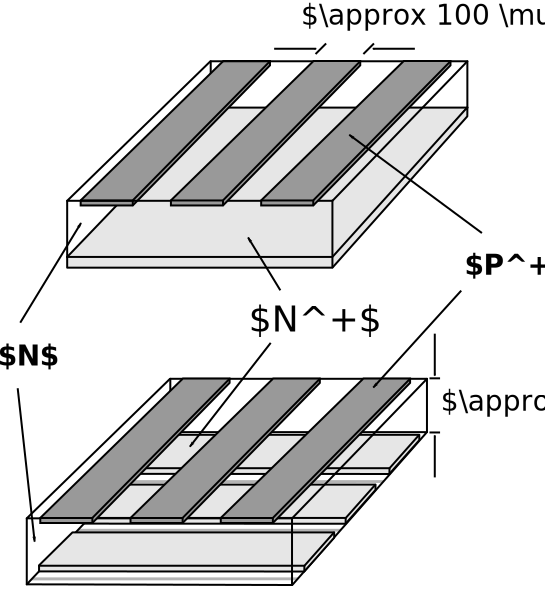
\includegraphics[width=\textwidth]{streifen.jpg}
			  \caption{Schema Streifendetektor [gsp]}
			\end{figure}
	    \column{.5\textwidth}
	    	\begin{itemize}
			  \item Meist n-dotiertes Grundmaterial mit p-dotierten Streifen
			  \item Streifenbreite 10-100 $\mu$m
			  \item einseitiger Streifendetektor $\rightarrow$ eindim. Ortsinformation
			  \item doppelseitig: Elektroden in nicht-parallele Streifen segmentieren (meist 90$^\circ$)
			  $\rightarrow$ zweidim. Ortsinformation
			\end{itemize}
    \end{columns}
\end{frame}


\begin{frame}{Pixeldetektoren}
	\begin{columns}[T]
		\column{.45\textwidth}
			\begin{figure}[htbp]
			  \centering
			  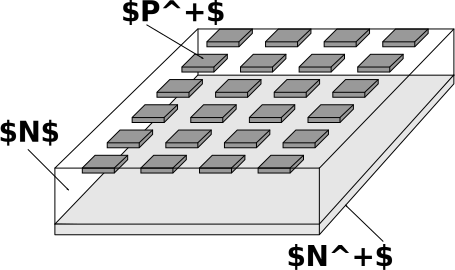
\includegraphics[width=\textwidth]{pixel.jpg}
			  \caption{Schema Pixeldetektor [gsp]}
			\end{figure}	
	    \column{.5\textwidth}
	    	\begin{itemize}
			  \item Elektroden in rechteckige Pixel segmentiert $\rightarrow$ zweidim. Ortsinformation
			  \item kleinere Elektrodenoberfläche besser um Signal zu verarbeiten (kleinerer Leckstrom)
			  \item hohe Kanalzahl
			\end{itemize}
    \end{columns}
\end{frame}


\begin{frame}{Pixeldetektoren}
			\begin{figure}[htbp]
			  \centering
			  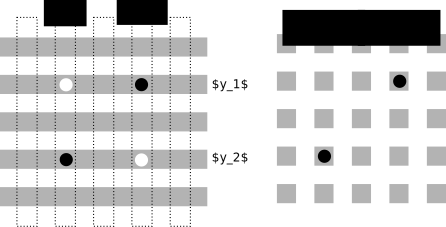
\includegraphics[width=\textwidth]{pixelstreifenvgl.jpg}
			  \caption{Mehrfachtreffer in doppelseitigem Streifendetektor erzeugen Mehrdeutigkeiten bei Zuordnung
			Trefferkoordinaten [gsp]}
			\end{figure}	
% 			 \vspace{1cm}			
\end{frame}


\begin{frame}{Pixel-/Streifendetektoren}
    \begin{columns}[T]
		\column{.45\textwidth}
			Vorteile		
			\begin{itemize}
			  \item gute Ortsauflösung $O(10\mu m)$  ($<$~MWPC/Driftkammer, aber Pixel~$<$~Streifen)
			  \item kleinere Energie, um $e^-$/Loch-Paar zu erzeugen $\rightarrow$ kleinere Variation der
			  Pulshöhe, höhere Energieauflösung
			  \item Pixeldetektoren erlauben eindeutige Zuordnung
			\end{itemize}	
	    \column{.5\textwidth}
	    	Nachteile
	    	\begin{itemize}
			  \item teuer
			  \item Kühlung notwendig, um Rauschen zu minimieren
			  \item begrenzte Haltbarkeit bei hoher Strahlung (nicht ionisierende Strahlung $\rightarrow$
			  z.B. Leerstellen im Gitter)
			\end{itemize}
    \end{columns}
   \end{frame}
   
%    \begin{frame}{Pixeldetektoren}
% 			\begin{figure}[htbp]
% 			  \centering
% 			  \includegraphics[width=\textwidth*0.5]{bla.jpg}
% 			  \caption{beispielbild}
% 			\end{figure}	
% % 			 \vspace{1cm}			
% \end{frame}